
\subsubsection{3.1 Dataset: OpenML Corpus}

The analysis uses the OpenML dataset corpus, a cross-sectional snapshot of N=5,217 datasets with at least one registered ML task ($N_{\text{tasks}}\geq 1$). OpenML \citep{Vanschoren2014OpenML} is a publicly accessible ML experimentation platform where researchers register datasets, define ML tasks, and execute experimental flows. The corpus was collected as of 2026-08-05 and preprocessed as a parquet file (\texttt{h-e1/results/preprocessed.parquet}).

\textbf{Sample restriction ($N_{\text{tasks}}\geq 1$):} This study examines conditional adoption intensity --- how tagging affects engagement among datasets that have received at least minimal engagement. Datasets with zero tasks are structurally different and would require a hurdle model component; this is deferred to future work. The sample restriction yields N=5,217 datasets: 2,625 tagged (50.3\%) and 2,592 untagged (49.7\%).

\textbf{Variables:}

\begin{table}[htbp]
\centering
\resizebox{\columnwidth}{!}{%
\begin{tabular}{lll}
\toprule
Variable & Role & Definition \\
\midrule
N\_tasks & Dependent variable & Count of distinct ML task registrations (integer $\geq$ 1) \\
has\_tags & Primary IV (P1) & Binary: 1 if dataset has $\geq 1$ keyword tag, 0 otherwise \\
log\_tag\_count\_p1 & Secondary IV (P2) & log(tag\_count + 1); restricted to has\_tags=1 subset \\
tag\_count\_cat & Categorical IV (P3) & Bins: 0, 1--2, 3--5, 6+ (reference: 0) \\
log\_n\_instances & Control & log(number of instances) \\
log\_n\_features & Control & log(number of features) \\
age\_years & Control & Dataset age in years \\
age\_sq & Control & $\text{age\_years}^2$ (quadratic age term) \\
C(decade) & Fixed effect & Decade-of-upload fixed effects \\
\bottomrule
\end{tabular}
}
\end{table}

\subsubsection{3.2 Model: Negative Binomial Type 2}

\textbf{Why NB-2 (not Poisson):} CT LR=7,356.36 (>> $\chi^{2}(1)=3.84$ critical value) confirms strong overdispersion across all three model specifications (CT LR=7,356.36 for P1; 7,357.39 for P2; 7,509.42 for P3). Poisson regression would underestimate standard errors and inflate significance.

\textbf{Why binary has\_tags rather than a composite score:} A prior episode on the same corpus tested a composite metadata completeness score (0--5). That composite yielded IRR=1.076 without decade fixed effects, collapsing to IRR=1.014 (p=0.19) under decade fixed effects. Binary has\_tags, by contrast, yields IRR=1.2263 and survives decade fixed effects with only 12.2\% attenuation. The binary variable isolates the FAIR F1 search-index-membership signal without dilution by non-F1 metadata fields.

\textbf{Why decade fixed effects:} Platform era shifts created extreme decade-tag collinearity (Cramér's V=0.823; nearly all 2010s datasets are tagged at a rate of 85.4\%, while 2020s datasets are tagged at only 2.1\%). C(decade) fixed effects control for between-era confounding. The structural character of the has\_tags effect --- its survival within decades --- is then verified via the mechanism test (Section 3.3).

All models were estimated using \texttt{statsmodels.formula.api.negativebinomial} with \texttt{loglike\textbackslash \_method='nb2'} and the BFGS optimizer (\texttt{method='bfgs'}, \texttt{maxiter=100}). Convergence was confirmed for all seven model variants. IRR = exp(coefficient); 95\% CI = $\exp(\text{coefficient} \pm 1.96\cdot SE)$.

\subsubsection{3.3 Four-Prediction Test Design}

\begin{table*}[htbp]
\centering
\resizebox{\dimexpr 2\columnwidth+\columnsep\relax}{!}{%
\begin{tabular}{lllll}
\toprule
Prediction & Model Formula & Sample & Gate Criterion & Gate Type \\
\midrule
P1 --- Binary Threshold & N\_tasks ~ has\_tags + controls + C(decade) & N=5,217 & $IRR\geq 1.1$, $CI_{\text{lower}}\geq 1.1$, p<0.05 & MUST\_WORK \\
Mechanism & P1 with vs. without C(decade) & N=5,217 & Post-FE $IRR\geq 1.1$, p<0.05 & MUST\_WORK \\
P2 --- Log-Linear & N\_tasks ~ log\_tag\_count\_p1 + controls + C(decade) & N=2,625 (tagged) & $CI_{\text{lower}}\geq 1.05$, p<0.05 & SHOULD\_WORK \\
P3 --- Categorical & N\_tasks ~ C(tag\_count\_cat) + controls + C(decade) & N=5,217 & Monotonic IRR, $\geq 2/3$ adjacent contrasts p<0.0167 & SHOULD\_WORK \\
\bottomrule
\end{tabular}
}
\end{table*}

Bonferroni correction for categorical contrasts: $\alpha =0.0167$ (k=3 contrasts). The mechanism test quantifies attenuation ratio = IRR\_without\_FE / IRR\_with\_FE; attenuation ratio < 1.5 constitutes STRONG mechanism support.

\begin{figure}[htbp]
\centering
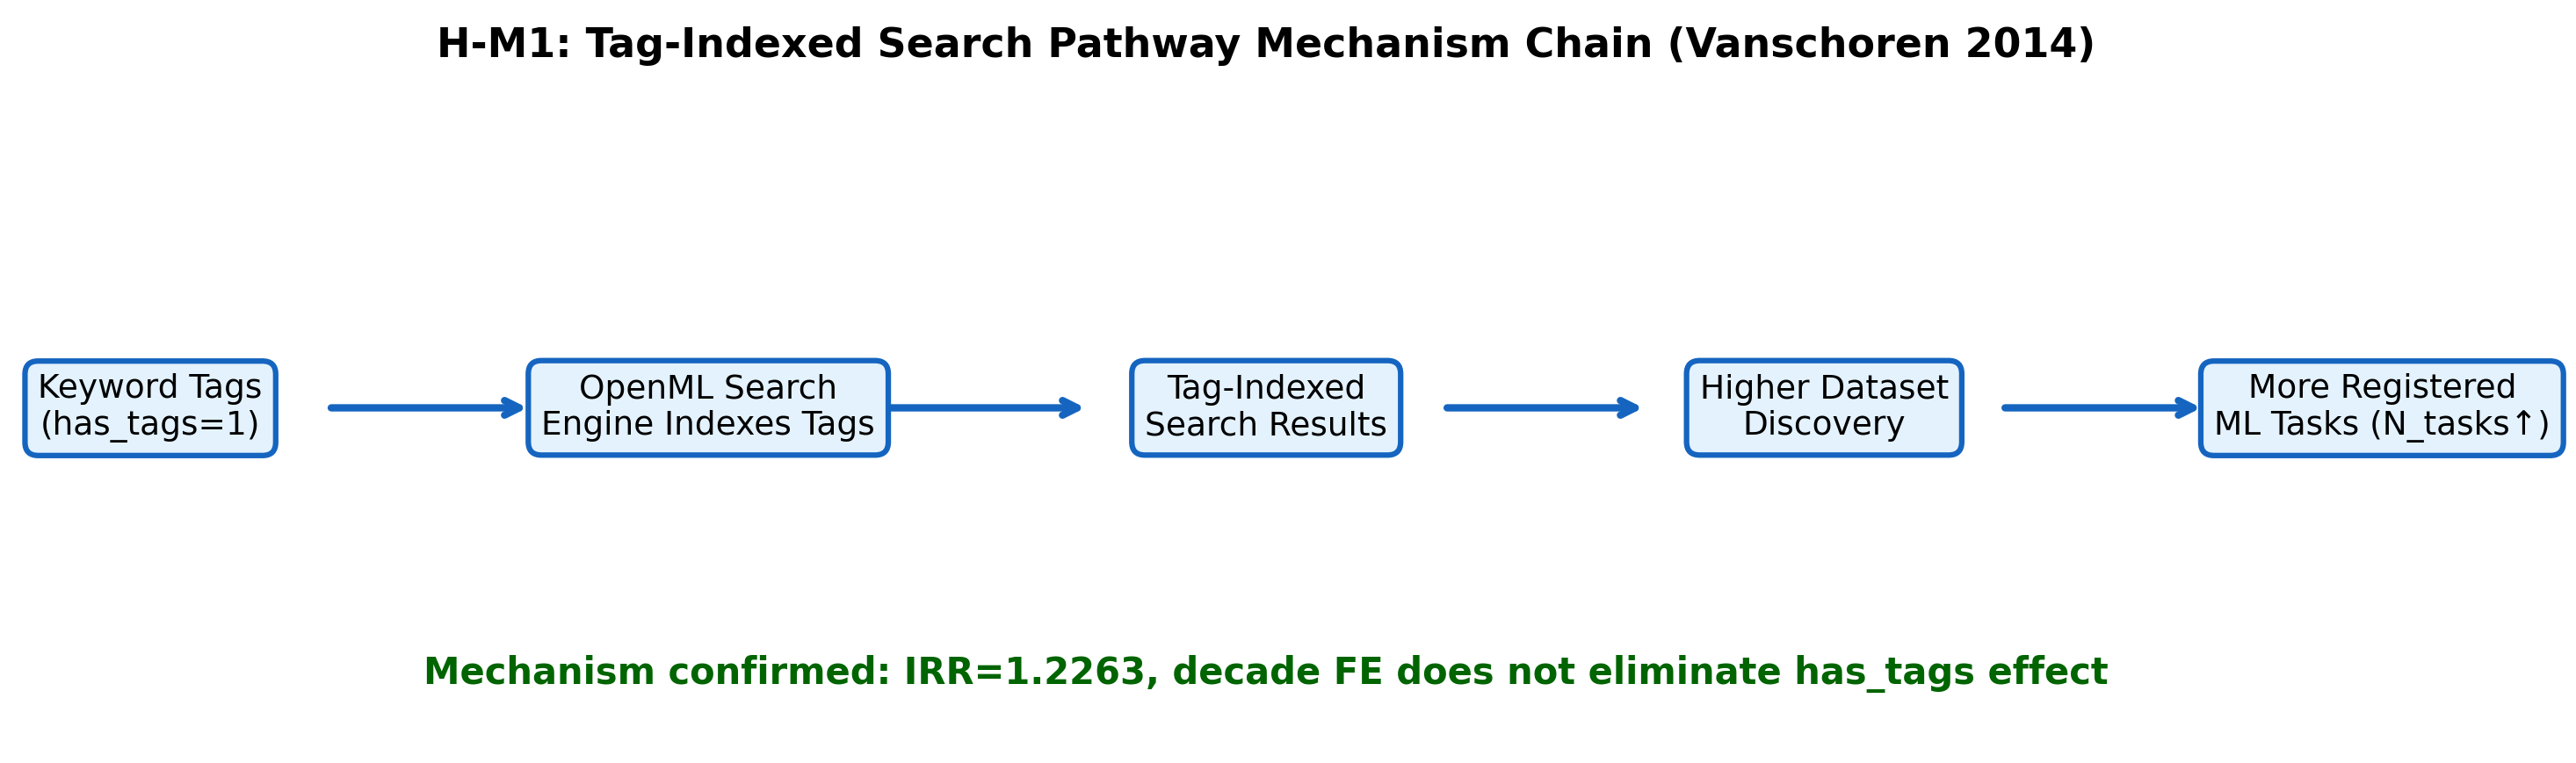
\includegraphics[width=\columnwidth]{figures/fig4_mechanism_flow.png}
\caption{FAIR F1 threshold-plus-amplification mechanism chain: Dataset keyword tags $\rightarrow$ search index membership $\rightarrow$ multiple search query pathways $\rightarrow$ researcher discovery events $\rightarrow$ ML task registration.}
\label{fig:fig4_mechanism_flow}
\end{figure}

\textit{Figure 1. FAIR F1 threshold-plus-amplification mechanism chain. Dataset keyword tags enable search index membership, which in turn expands the set of search query pathways through which researchers encounter the dataset, ultimately driving ML task registration. Source: h-m1/figures/fig4\_mechanism\_flow.png.}

\subsubsection{3.4 Robustness Checks}

Pre-specified robustness checks include: RC-4 (winsorize N\_tasks at the 99th percentile), RC-7 (age-only control versus decade fixed effects sensitivity comparison), and the mechanism attenuation test (with/without C(decade) fixed effects for P1). RC-5 (tagged-only subset for has\_tags) was pre-specified but is not applicable because has\_tags is constant (=1) in the tagged subset; this was noted as an expected design limitation.

